% !TEX root = ../main.tex

\chapter{实现与评估} \label{ch:implement}

\section{编译链及定理证明的实现}

如第~\ref{sec:overview}节中所述,我们主要使用了交互式定理证明器Coq实现
程序语言定义及编译算法,并完成相关定理的形式化证明。
Coq主要是用OCaml语言实现的,它支持数学断言的表示,并且能够检查这些断言的证明,
从其形式化的构造证明中提取出验证程序~\cite{paulin2011introduction}。
作为一种编程语言,Coq是一种依赖类型的函数式编程语言;作为一种逻辑系统,它实现了一种高阶类型理论。
也就是说,证明即是程序。

其中,编译链的PCF语法分析器(Parser)部分在OCaml中实现,它分析PCF程序文本并
在顶层Coq模块中添加需要进行编译的PCF源程序。我们在本章第~\ref{sec:pcfparser}节对其进行了介绍。
我们在Coq中完成了PCF、CPS和SSA程序语言的定义以及从PCF源程序到Vellvm抽象语法树的编译链。
这些编译过程和证明主要通过函数和模式匹配(Pattern Match)、
表示推理规则的归纳类型(Inductive)、一阶逻辑(First-Order Logic)谓词等实现。
Coq并没有提供通常的原子数据类型(布尔值、整数、字符串等),而是提供了一个机制来定义新的数据类型。
当然,Coq有强大的标准库,其中包含了许多常见数据结构的定义。
在后文中我们会详细介绍在Coq中对经验证编译链进行实现的过程。

\subsection{PCF语法分析器} \label{sec:pcfparser}
我们没有直接去编写实现词法解析和语法解析功能的OCaml代码,而是
使用ocamllex和ocamlyacc~\cite{smith2007ocamllex}作为词法和语法解析器的生成器。
它们的用法类似于C语言环境中的lex和yacc~\cite{levine1992lex}。
该PCF语法分析器的结构如图~\ref{fig:parser}所示。

Ocamllex可以从附加了语义行为的正则表达式(Regular Expression)集合中生成词法分析器。
我们首先在\textit{lexer.mll}中定义了直接风格PCF语言的词法解析规则,
包括输入文本中各种词法单元的模式匹配和对应的操作,然后使用ocamllex
生成词法分析器的OCaml代码\textit{lexer.ml}。
在\textit{lexer.ml}文件中,词法分析函数将词法分析缓冲区(Lexer Buffer)作为参数,
生成标记流(Tokens)。
词法分析缓冲区是在OCaml标准库模块Lexing中实现的抽象数据类型,它维护分析函数当前的状态,
并可以从输入获取内容对缓冲区进行填充~\cite{leroy2021ocaml}。
分析函数会将缓冲区中的字符与词法规则中定义的正则表达式进行匹配,直到输入的前缀符合某条规则,
执行相应的操作。如果符合多条规则,就按照最长匹配原则。
Ocamlyacc会根据语法规则\textit{grammar.mly}生成语法分析器的接口\textit{grammar.mli}
和实现\textit{grammar.ml}。语法解析函数的参数包括上文中提到的词法分析器和词法分析缓冲区。
它将词法分析得到的标记流解析为抽象语法树。之后,我们使用\textit{printer.ml}读入PCF程序
在OCaml中的抽象语法树打印出它的Coq程序并将其写入Coq编译链的顶层模块,这样就可以直接在Coq中使用它了。

\begin{figure}[htbp]
    \centering
    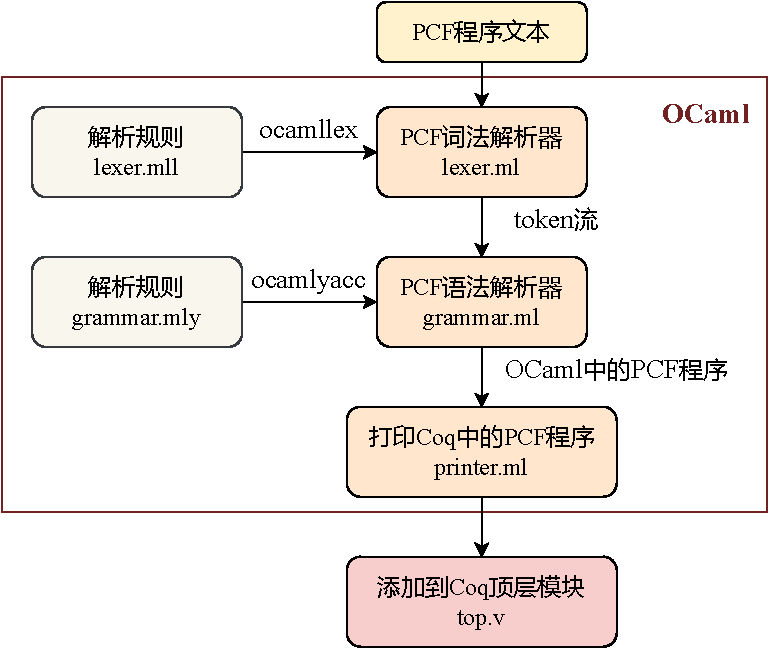
\includegraphics[width=0.7\linewidth]{figures/pcfparser.pdf}
    \caption{PCF语法分析器结构}\label{fig:parser}
\end{figure}

\subsection{程序语言定义}

如上一节所述,我们已经使用PCF语法分析器在Coq顶层编译模块得到了PCF程序的抽象语法树。
除了PCF语言的抽象语法树定义,我们还为其在Coq中实现了第~\ref{sec:cps}节中定义的小步操作语义。
我们使用Inductive类型完成了这种程序状态转换规则的定义。

\begin{lstlisting}[language=Coq]
    Inductive  pcf_term : Set  := ...
    Record  pcf_state  :=  mk_state {t : pcf_term;  ctx : context;}.
    Inductive  pcf_step : pcf_state -> pcf_state -> Prop  := ...
\end{lstlisting}

在编译算法正确性证明过程中使用的小步操作语义是关系型的,即表示为两个程序状态之间的关系。
这样的设计对于证明来说很方便,但是无法直接运行程序得到结果。
为了对操作语义和转换算法进行初步测试,使用Coq为三种语言分别构建解释器(Interpreter),
从而能够执行相应的程序,得到程序返回的结果。其中,发散的定义要取决于对最大步数的限定,即解释器的fuel。
解释器每走一步都会消耗一个fuel,如果fuel消耗完程序还没有终止或出错,就可以认为程序发散了,返回超时状态(Timeout)。
进行解释器测试主要是为了找出操作语义和转换算法中的问题,为接下来的证明减少阻碍。形式化验证过程本身与解释器没有关系。

\begin{lstlisting}[language=Coq]
    Inductive  pcf_result : Type  := 
        |  terminate : nat  ->  pcf_result 
        |  error : pcf_result
        |  timeout : pcf_result
    Fixpoint  pcf_interpreter  (fuel : nat)  (state : pcf_state) : 
        pcf_result  :=  let  'mk_state  term ctx  :=  state  in
                            match fuel with 
                                | 0  =>  timeout 
                                | S fuel'  =>  match  term, ctx  with ...
\end{lstlisting}

与PCF语言类似,我们为CPS与SSA语言也像这样完成了其语法、语义及解释器在Coq中的实现。

\subsection{转换算法的实现}

CPS转换算法~\ref{algo:cpstrans}和CPS到SSA的转换算法~\ref{cps2ssa}均在Coq中进行实现。
对于CPS转换,我们需要根据已有的变量名称列表生成新变量,且新变量不能与已有的变量名重复。
在具体实现时,我们采用的算法是为新生成的变量维护一个后缀最大值$n$。
当需要生成一个新的变量名时,我们首先尝试将前缀字符串后连接后缀$n$,并将后缀最大值加一。
这样一个字符串虽然不会与新生成的变量名冲突,但是可能会和CPS程序原有的变量名冲突。
由于我们的CPS转换算法会持续记录已有的变量名列表$l_v$,我们还需要使之与$l_v$中的
变量比较。如果产生冲突,需要重复上一步。
对于CPS到SSA的转换算法,我们首先需要实现插入指令、基本代码块、函数的$\mathbf{app}$操作。
然后,我们需要能够根据已处理的条件语句数量$n$生成新的基本代码块标签的操作fresh\_block\_label。
之后,我们就可以实现~\ref{sec:cpsssatrans}节中的转换算法了。

\begin{lstlisting}[language=Coq]  
    Definition  app_i  (i : instruction)  (t : ssa_term)  (p : pc)  : 
        ssa_term  := ... 
    Definition  fresh_block_label  (n : nat)  :  string  := ...
    Definition  G_state  :  Type  :=  (ssa_term  *  nat  *  loc_cps).
    Fixpoint  G  (t_cps : cps_term)  (t_ssa : ssa_term)  (p : pc)  
        (n : nat)  (loc : loc_cps)  :  G_state  := ...
    Definition  G_prog  (t_cps : cps_term)  :  ssa_term  := ...
\end{lstlisting}

我们还实现了从SSA到Vellvm抽象语法树的编译过程。
将Vellvm作为子模块使用,该转换步骤的目标语言是Vellvm在\textit{Syntax.LLVMAst}文件中定义的LLVM IR。
正如我们在介绍SSA语言时所说,该SSA保留了LLVM IR程序的结构。
此步转换主要是进行结构上的映射,顺便为被省略的参数选取正确的默认值。
例如,我们可以直接把SSA中的函数调用指令$x = \mathbf{call}\; f\; v$转换为LLVM AST中的
INSTR\_Op指令,但是需要为其指定$f$和$v$的类型。在这里我们统一使用64位无符号整型。
其他结构同理,基本代码块转换为LLVMAst.block,函数转换为definition,顶层翻译单元转换为toplevel\_entities。

得到Vellvm中的抽象语法树后,就可以利用其提供的工具进行LLVM程序的输出或使用LLVM后续的编译过程了。

\subsection{定理证明的实现}

\section{Coq代码评估}

各主要模块类别和内容的代码行数(Lines of Code, LOC)如下表~\ref{tabeval}。可以看到,相关定理的证明即转换算法验证部分是工作量占比最大的。

\begin{table}
    \linespread{1.25}
    \small
    \centering
    % \vspace{-20pt}
    \caption{Coq代码LOC评估}\label{tabeval}
    \begin{center}
    \begin{tabular}{|l|l|l|l|}
    \hline
    代码类别 & 代码实现内容 & LOC & 行数占比(\%) \\
    \hline
    \multirow{3}{*}{程序语言定义} & PCF & 171 & \multirow{3}{*}{23.9} \\
        & CPS & 228 & \\
        & SSA & 303 & \\
        \hline
    \multirow{3}{*}{转换算法} & PCF$\rightarrow$CPS & 148 & \multirow{3}{*}{24.5} \\
        & CPS$\rightarrow$SSA & 251 & \\
        & SSA$\rightarrow$LLVM IR & 318 & \\
        \hline
    \multirow{4}{*}{形式化验证} & PCF$\rightarrow$CPS前向模拟 & 364 & \multirow{4}{*}{51.6} \\
        & CPS$\rightarrow$SSA前向模拟 & 696 & \\
        & 前向模拟组合 & 49 & \\
        & 后向模拟 & 404 & \\
        \hline
    \end{tabular}
    \end{center}
\end{table}

